\cotefile{156-8}
\scanpage{121}
\mspage{112}
% archive sheet number: 121

Regardons l'opération \unsure{suiv.} $\unsure{A}$ sur $\Phi$
\diagram{
\footnotesize
\begin{tikzcd}[ampersand replacement=\&,column sep=small,row sep=small]
\Phi \arrow[r,mapsto] \&
\overline{\Phi} \arrow[r,mapsto] \&
\underbrace{\overline{\Phi}\setminus\underset{\substack{\Vert\\\Phi_{\mathrm{is}}}}{\overline{\Phi}_{\mathrm{is}}}}_{\substack{\text{adhérence}\\\text{purement}\\\text{1-dimensionnelle}}}
\arrow[r,mapsto,double,shorten <=2pt] \&
\Phi_{\deleted{\unsure{\mathrm{t\acute elescope}}}\mathrm{conv}}=\boxed{\Psi}
\\
\& \begin{gathered}\text{\uline{figure}}\\
\text{\uline{\unsure{enveloppante}}}\\
\deleted{\unsure{\mathrm{associ\acute ee}}}\deleted{\unsure{\Phi}}\ \text{de}\\
\Phi,\ \text{\uline{ou adhérence}}
\end{gathered}
\&
\& \begin{gathered}\text{ou ``\deleted{\unsure{télescopage}}}\\
\text{\inserted{\unsure{complétion|contraction}}}\\
\text{par effacement}\\\text{des pts ordinaires}\\
\text{de }\overline{\Phi}\setminus\overline{\Phi}_{\mathrm{is}}\text{''}
\end{gathered}
\end{tikzcd}}

On trouve une figure dont les composantes connexes sont des segments, donc donnée par une \deleted{suite} drapeau dans $\unsure{\mathcal{M}|M}_1$, ordonné par $\deleted{\unsure{\lhd}}\lhd$
\[
\begin{aligned}
D&\in\mathrm{Drap}^{*}(\mathcal{M}_1,\lhd)\\
\Big\Vert\quad&\\[-1.5ex]
\{X_1,X_2,\ldots X_n\}&
\end{aligned}
\]
\[
\text{\unsure{``}}\qquad X_i=\unsure{S|\mathscr{S}}_{a_i,b_i}\,,
\]
\figure{
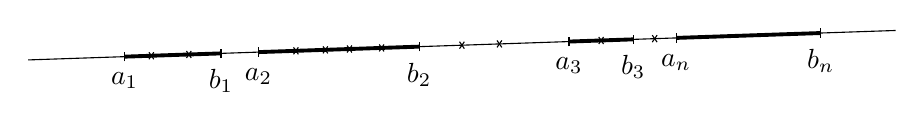
\begin{tikzpicture}[x=.68cm,y=.68cm]
\draw[thin] (0,0)--(16.2,.55);
\draw[line width=1.4pt] (1.8,.061)--(3.6,.122);
\draw[line width=1.4pt] (4.3,.146)--(7.3,.248);
\draw[line width=1.4pt] (10.1,.343)--(11.3,.384);
\draw[line width=1.4pt] (12.1,.411)--(14.8,.502);
\foreach \x/\y/\lab in {1.8/.061/a_1,3.6/.122/b_1,4.3/.146/a_2,7.3/.248/b_2,10.1/.343/a_3,11.3/.384/b_3,12.1/.411/a_n,14.8/.502/b_n}{
\draw (\x,\y-.09)--(\x,\y+.09);
\node[below] at (\x,\y-.12) {$\lab$};}
\foreach \x/\y in {2.3/.078,3/.102,5/.17,5.55/.188,6/.204,6.6/.224,8.1/.275,8.8/.299,10.7/.363,11.7/.397}{
\draw (\x-.045,\y-.065)--(\x+.045,\y+.065);
\draw (\x-.045,\y+.065)--(\x+.045,\y-.065);}
\end{tikzpicture}}

de telle façon que
\[
\left\{\begin{aligned}
\Psi=\Phi_{\mathrm{conv}}&=\Phi_D=\Phi_{X_1,X_2,\ldots,X_n}\\
\delta\deleted{\unsure{\Phi}}\Psi_{\deleted{\unsure{\mathrm{conv}}}}\inserted{{}=\delta\Psi}&=\partial\Phi=\{a_1,b_1,a_2,b_2,\ldots,a_n,b_n\}.
\end{aligned}\right.
\]

Pour \deleted{en donner} décrire $\Phi$ en termes de $\Phi_{\deleted{\unsure{\mathrm{comp}|\mathrm{conv}}}\mathrm{conv}}$ il faut :

1°) Donner $\inserted{\boxed{\Delta}}\unsure{\delta|\partial}\Phi=\ \in\mathrm{Drap}^{*}(\unsure{\mathcal{L}|L})\supset\unsure{\delta|\partial}\Psi$

\hspace*{1em}drapeau de $\mathcal{L}$ contenant $\delta\Psi$.

Les nouveaux pts rajoutés\textsuperscript{*} sont donc \unsure{juste} les \deleted{points} sommets isolés et les sommets internes de $\Phi$.
% slanted
\margin{\textsuperscript{*}\unsure{marqués} par un $\times$}
